\newcommand{\SystemFigure}{%
\begin{figure*}[t]
\centering
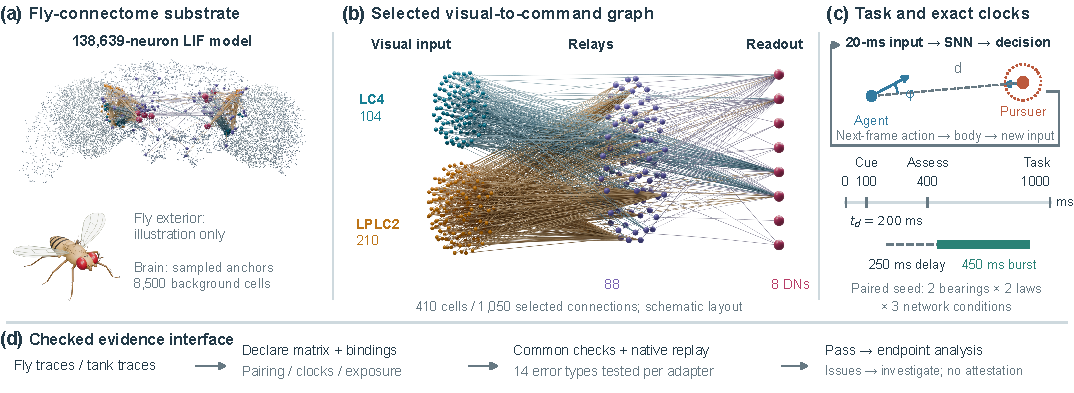
\includegraphics[width=\textwidth]{figs/evidence_v10_overview_parenthesized.pdf}
\caption{System and checked assessment interface. (a) Model anchors and an illustrative fly; (b) schematic 410-cell/1,050-connection graph, not measured neurites or the full recurrent network. (c) Sampled feedback and exact burst events; $t_d=200$\,ms is illustrative. (d) Common checks and native replay; the 14 types are development challenges, separate from Fig.~\ref{fig:v10f-reuse}'s catalogue.}
\label{fig:v10f-system}
\end{figure*}}
\newcommand{\ReuseCaption}{Cross-plant example and frozen-checker ablation. (a) First tank seed, high inflow, proportional law; zoomed level axis, safe interval $[0.2,0.8]$; all 96 tasks remain safe. (b) Requested outflow at 0.60\,s applies at 0.75\,s on 100-ms frames. (c) Invalid cases detected: A headers, B=A+common, C=A+native, D=full. Fly/tank invalid denominators are 45/42, with 12 valid controls each. Designed cases are not general coverage.}
\newcommand{\WarningCaption}{Frozen secondary warning operating points. Rows state contact/success denominators; RF-0/A/B contain 24/12/12 independent seed clusters. Markers show (a) missed-contact and (b) false-alarm rates with pointwise 95\% whole-seed bootstrap CIs. Activity is two-sided; the forecast holds the current command using exact simulated state. Positive-class support is 12/2/1 seed clusters. Zero-width and class-conditional empirical intervals do not establish zero population risk.}
\iffourfigures
\newcommand{\reuseRef}{Fig.~\ref{fig:v10f-reuse}}
\newcommand{\warningRef}{Fig.~\ref{fig:v10f-warning}}
\newcommand{\ReuseFigure}{%
\begin{figure}[t]\centering
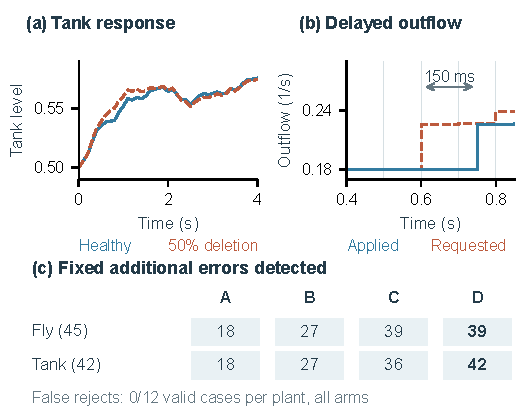
\includegraphics[width=\columnwidth]{figs/v10_1_ablation.pdf}
\caption{\ReuseCaption}\label{fig:v10f-reuse}
\end{figure}}
\newcommand{\WarningFigure}{%
\begin{figure}[t]\centering
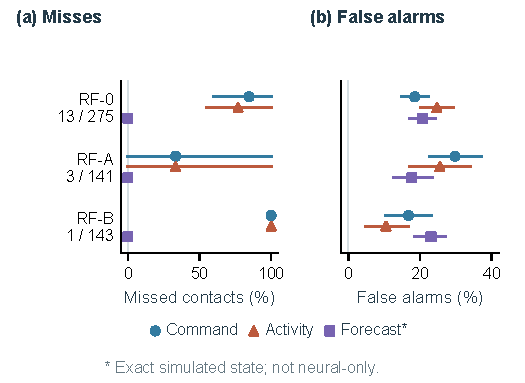
\includegraphics[width=\columnwidth]{figs/v10_1_warning_count.pdf}
\caption{\WarningCaption}\label{fig:v10f-warning}
\end{figure}}
\else
\newcommand{\reuseRef}{Fig.~\ref{fig:v10f-reuse} (left)}
\newcommand{\warningRef}{Fig.~\ref{fig:v10f-warning} (right)}
\newcommand{\ReuseFigure}{%
\begin{figure*}[t]\centering
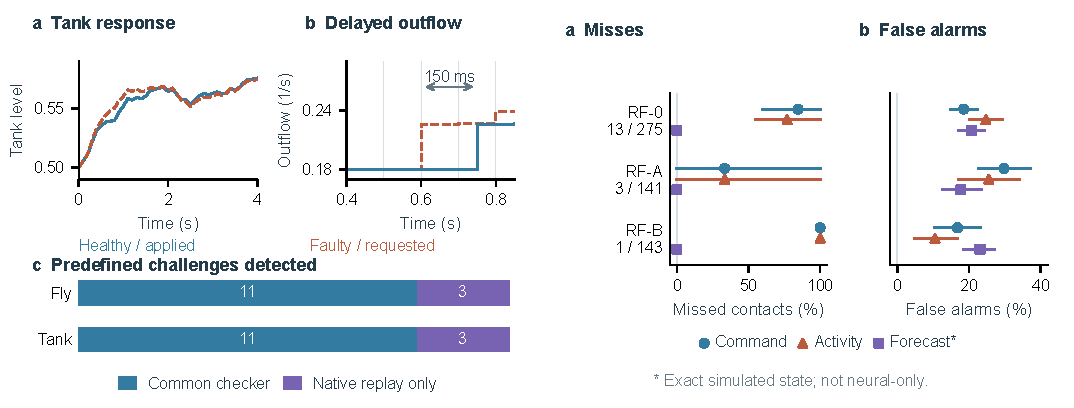
\includegraphics[width=\textwidth]{figs/v10f_reuse_warning.pdf}
\caption{\emph{Left:} \ReuseCaption\ \emph{Right:} \WarningCaption}
\label{fig:v10f-reuse}\label{fig:v10f-warning}
\end{figure*}}
\newcommand{\WarningFigure}{}
\fi
\newcommand{\TransferFigure}{%
\begin{figure*}[t]\centering
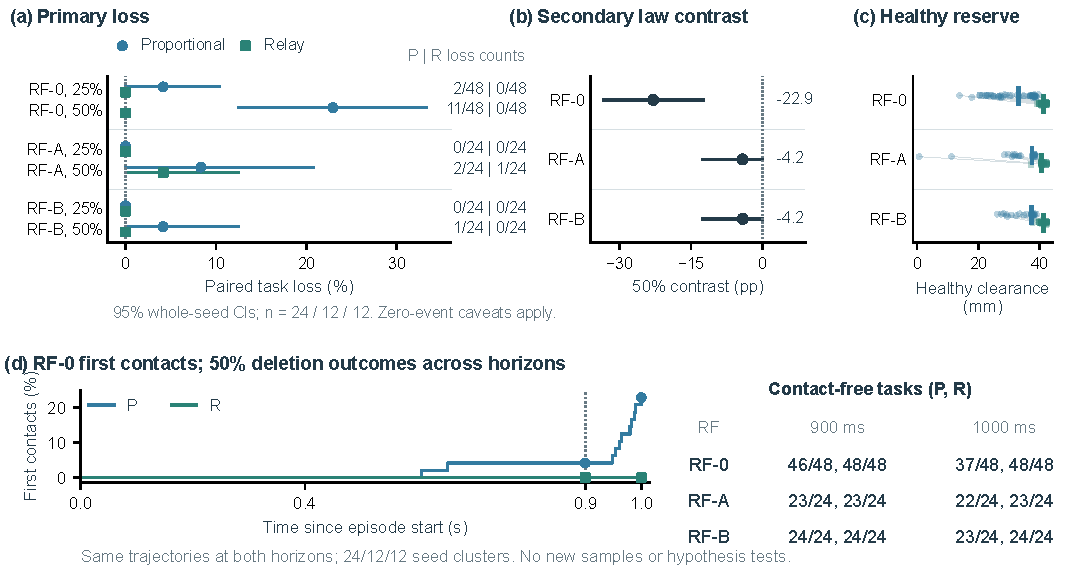
\includegraphics[width=\textwidth]{figs/v10h_rf_parenthesized.pdf}
\caption{Paired loss across sensory realizations and horizons. (a) Primary losses and (b) prespecified secondary R-minus-P contrasts (percentage points), with pointwise 95\% whole-seed CIs, $n=24/12/12$, conditional on saved calibrations. All healthy tasks succeed; no gains occur. (c) Paired healthy minimum-clearance points and median marks show unequal reserve. (d) RF-0/50\% first contacts and all-map 900/1000-ms success counts (P, R); both endpoints reuse the same 24/12/12 seed clusters, not new replicates or tests. Maps differ in draws, recalibration and cohorts, not an isolated RF effect.}
\label{fig:v10f-transfer}
\end{figure*}}
